\documentclass[12pt]{article}
%% Useful packages
\usepackage{fontspec}
\setmainfont{Times New Roman}
\usepackage[francais]{babel}
\usepackage[a4paper,left=2cm,right=2cm,top=2cm,bottom=2cm]{geometry}
\usepackage{crop,graphicx,amsmath,array,color,amssymb,fancyhdr,lineno}
\usepackage{flushend,stfloats,amsthm,chngpage,times,,lipsum,lastpage} 
\usepackage{calc,listings,color,wrapfig,tabularx,longtable,enumitem}
\usepackage[style=numeric-comp,backend=biber]{biblatex}
\addbibresource{Refs.bib}
\usepackage{lineno}
\usepackage{hyperref}
\usepackage[utf8]{inputenc}\usepackage{algorithm}
\usepackage{vhistory}
\usepackage{algorithmic}
\usepackage{tikz}
\usepackage{etoc}
\renewcommand*\contentsname{Summary}

%%%%%%%%%%%%   Header and Footer  %%%%%%%%%%%%%
\pagestyle{fancy}
\fancypagestyle{plain}{%
  \renewcommand{\headrulewidth}{0pt}%j
  \fancyhf{}%
}

\title{%
 Application de gestion de portefeuille}
\author{CHÉMERY Julien \\
\\
MERBOUCHE Mouloud
\\ 
TEBOUL Elisa}

\begin{document}
\begin{titlepage}

\newcommand{\HRule}{\rule{\linewidth}{0.5mm}} % Defines a new command for the horizontal lines, change thickness here

%----------------------------------------------------------------------------------------
%	LOGO SECTION
%----------------------------------------------------------------------------------------
\center

\includegraphics[width=5cm]{Title/logoISEP.png}\\[1cm] % Include a department/university logo - this will require the graphicx package
 
%----------------------------------------------------------------------------------------

\center % Center everything on the page

%----------------------------------------------------------------------------------------
%	HEADING SECTIONS
%----------------------------------------------------------------------------------------

\textsc{\LARGE \underline{Institut Supérieur d'Électronique de Paris}} \\[1.5cm] % Name of your university/college
\textsc{\Large Algorithmique et programmation}\\[0.5cm] % Major heading such as course name
    \textsc{\Large Cycle ingénieur (A1)}\\[0.05cm]


%----------------------------------------------------------------------------------------
%	TITLE SECTION
%----------------------------------------------------------------------------------------
\makeatletter
\HRule \\[0.4cm]
{ \huge \bfseries \@title}\\[0.4cm] % Title of your document
\HRule \\[1.5cm]
 
%----------------------------------------------------------------------------------------
%	AUTHOR SECTION
%----------------------------------------------------------------------------------------

\begin{minipage}{0.4\textwidth}
\begin{flushleft} \large
\emph{\underline{Étudiants}:}\\
\@author % Your name
\\[1.2em]
\emph{\underline{Code module}: IR.1101}\\

\end{flushleft}
\end{minipage}
~
\begin{minipage}{0.4\textwidth}
\begin{flushright} \large
\emph{\underline{Groupe}:} \\
Émoulien \\[1.2em] % Supervisor's Name

\emph{\underline{Encadrant}:} \\
ALLANIC Hervé% second marker's name
\end{flushright}
\end{minipage}\\[2cm]
\makeatother

% If you don't want a supervisor, uncomment the two lines below and remove the section above
%\Large \emph{Author:}\\
%John \textsc{Smith}\\[3cm] % Your name

%----------------------------------------------------------------------------------------
%	DATE SECTION
%----------------------------------------------------------------------------------------

{\large \today}\\[2cm] % Date, change the \today to a set date if you want to be precise

\vfill % Fill the rest of the page with whitespace

\end{titlepage}

\sffamily

\fancyhf{}
\fancyhead[L]{Projet JavaFX}
\fancyhead[R]{}
\fancyfoot[R]{ \bf\thepage\ \rm }%

\newpage


\pagebreak

\tableofcontents

\thispagestyle{empty}

\listoffigures

\newpage

\section{Présentation du sujet}

Le projet II.1102 de cette année consiste à développer une application graphique de gestion de portefeuille financier en Java. Cette application permettra de suivre les valeurs d'un ou plusieurs portefeuilles au fil du temps, qu'il s'agisse d'actions ou de cryptomonnaies. L'application doit répondre à des exigences et pour ce faire utilise deux API publiques : Coin Gecko (limité à 5 messages par minute) et Alpha Vantage (limité à 25 requêtes par jour).

\section{Fonctionnalités de notre application}

Les fonctionnalités sont les suivantes :

\begin{enumerate}
    \item Compte \begin{enumerate}
        \item [\tiny$\bullet$] Création : L'utilisateur peut créer un compte en renseignant son nom et un mot de passe complexe.
        \item [\tiny$\bullet$] Connexion : L'utilisateur pourra ensuite se connecter avec le compte qu'il a crée.
    \end{enumerate}
    \item Portefeuille\begin{enumerate}
        \item [\tiny$\bullet$] Création : L'utilisateur peut créer des portefeuilles avec des noms différents.
        \item [\tiny$\bullet$] Suppression : Il est possible de supprimer un portefeuille parmi ceux créées.
        \item [\tiny$\bullet$] Duplication : Il peut dupliquer un portefeuille existant, en conservant les informations relatives aux cryptomonnaies et actions, mais en remettant les quantités à 0.
        \item [\tiny$\bullet$] Rechargement : L'utilisateur peut recharger son compte avec de l'argent, qui sera ensuite disponible pour pouvoir acheter avec ses portefeuilles.
        \item [\tiny$\bullet$] Historique : L'utilisateur a accès à un historique de transaction global pour son compte qui lui permettra de voir toutes les actions et cryptos d'une vue globale.
    \end{enumerate}
    \item Actions / Cryptomonnaies \begin{enumerate}
        \item [\tiny$\bullet$] Achat : L'utilisateur peut acheter des actions ou des cryptomonnaies en renseignant le nombre d'unité à acheter et pourra voir le prix actuel de celle-ci. 
        \item [\tiny$\bullet$]Vente : Il est possible de vendre des actions ou des cryptomonnaies, la plus-value ou la perte sera ajoutée ou déduit du solde de l'utilisateur.
        \item [\tiny$\bullet$] Recherche de cryptos : L'utilisateur peut recharger parmi la base de donné de l'API (Coin Gecko) la valeur d'une cryptomonnaies. 
        \item [\tiny$\bullet$] Recherche d'actions : L'utilisateur peut rechercher, parmi la base de donné de l'API Alpha Vantage, une entreprise (avec un mot clé, par exemple Nvidia au lieu de NVDA) pour avoir la valeur d'une action.
    \end{enumerate}
    \item Affichage \begin{enumerate}
        \item [\tiny$\bullet$] La visualisation de l'historique d'une cryptomonnaie (BTC et ETH), nous pouvons voir l'historique en fonction de différentes années, avec la valeur réelle affichée pour l'année en cours sur le graphique.
        \item [\tiny$\bullet$] L'Affichage d'un camembert indiquera la répartition d'actions et de cryptomonnaies au sein d'un portefeuille en terme de quantité.
    \end{enumerate}
    \item Sauvegarde \begin{enumerate}
        \item [\tiny$\bullet$] L'application permet de sauvegarder automatiquement chaque portefeuille, chaque transaction et tout les éléments d'un compte.
    \end{enumerate}
\end{enumerate}



\newpage

\section{Diagramme UML}
Les diagrammes UML nous ont d'abord permis de pouvoir s'orienter de façon plus précise pour la partie réalisation du projet. Nous avons choisi pour cette partie d'afficher uniquement le diagramme UML contenant, les constructeurs et les variables. Ce choix est justifié par des raisons de simplicité pour le rapport. En effet, l'ajout des méthodes rend la taille du diagramme beaucoup trop grande. Toutefois, les autres diagrammes UML sont toujours disponibles à l'adresse suivante : \href{https://ibb.co/WnzWVmF}{UML}.
\begin{figure}[H]
    \centering
    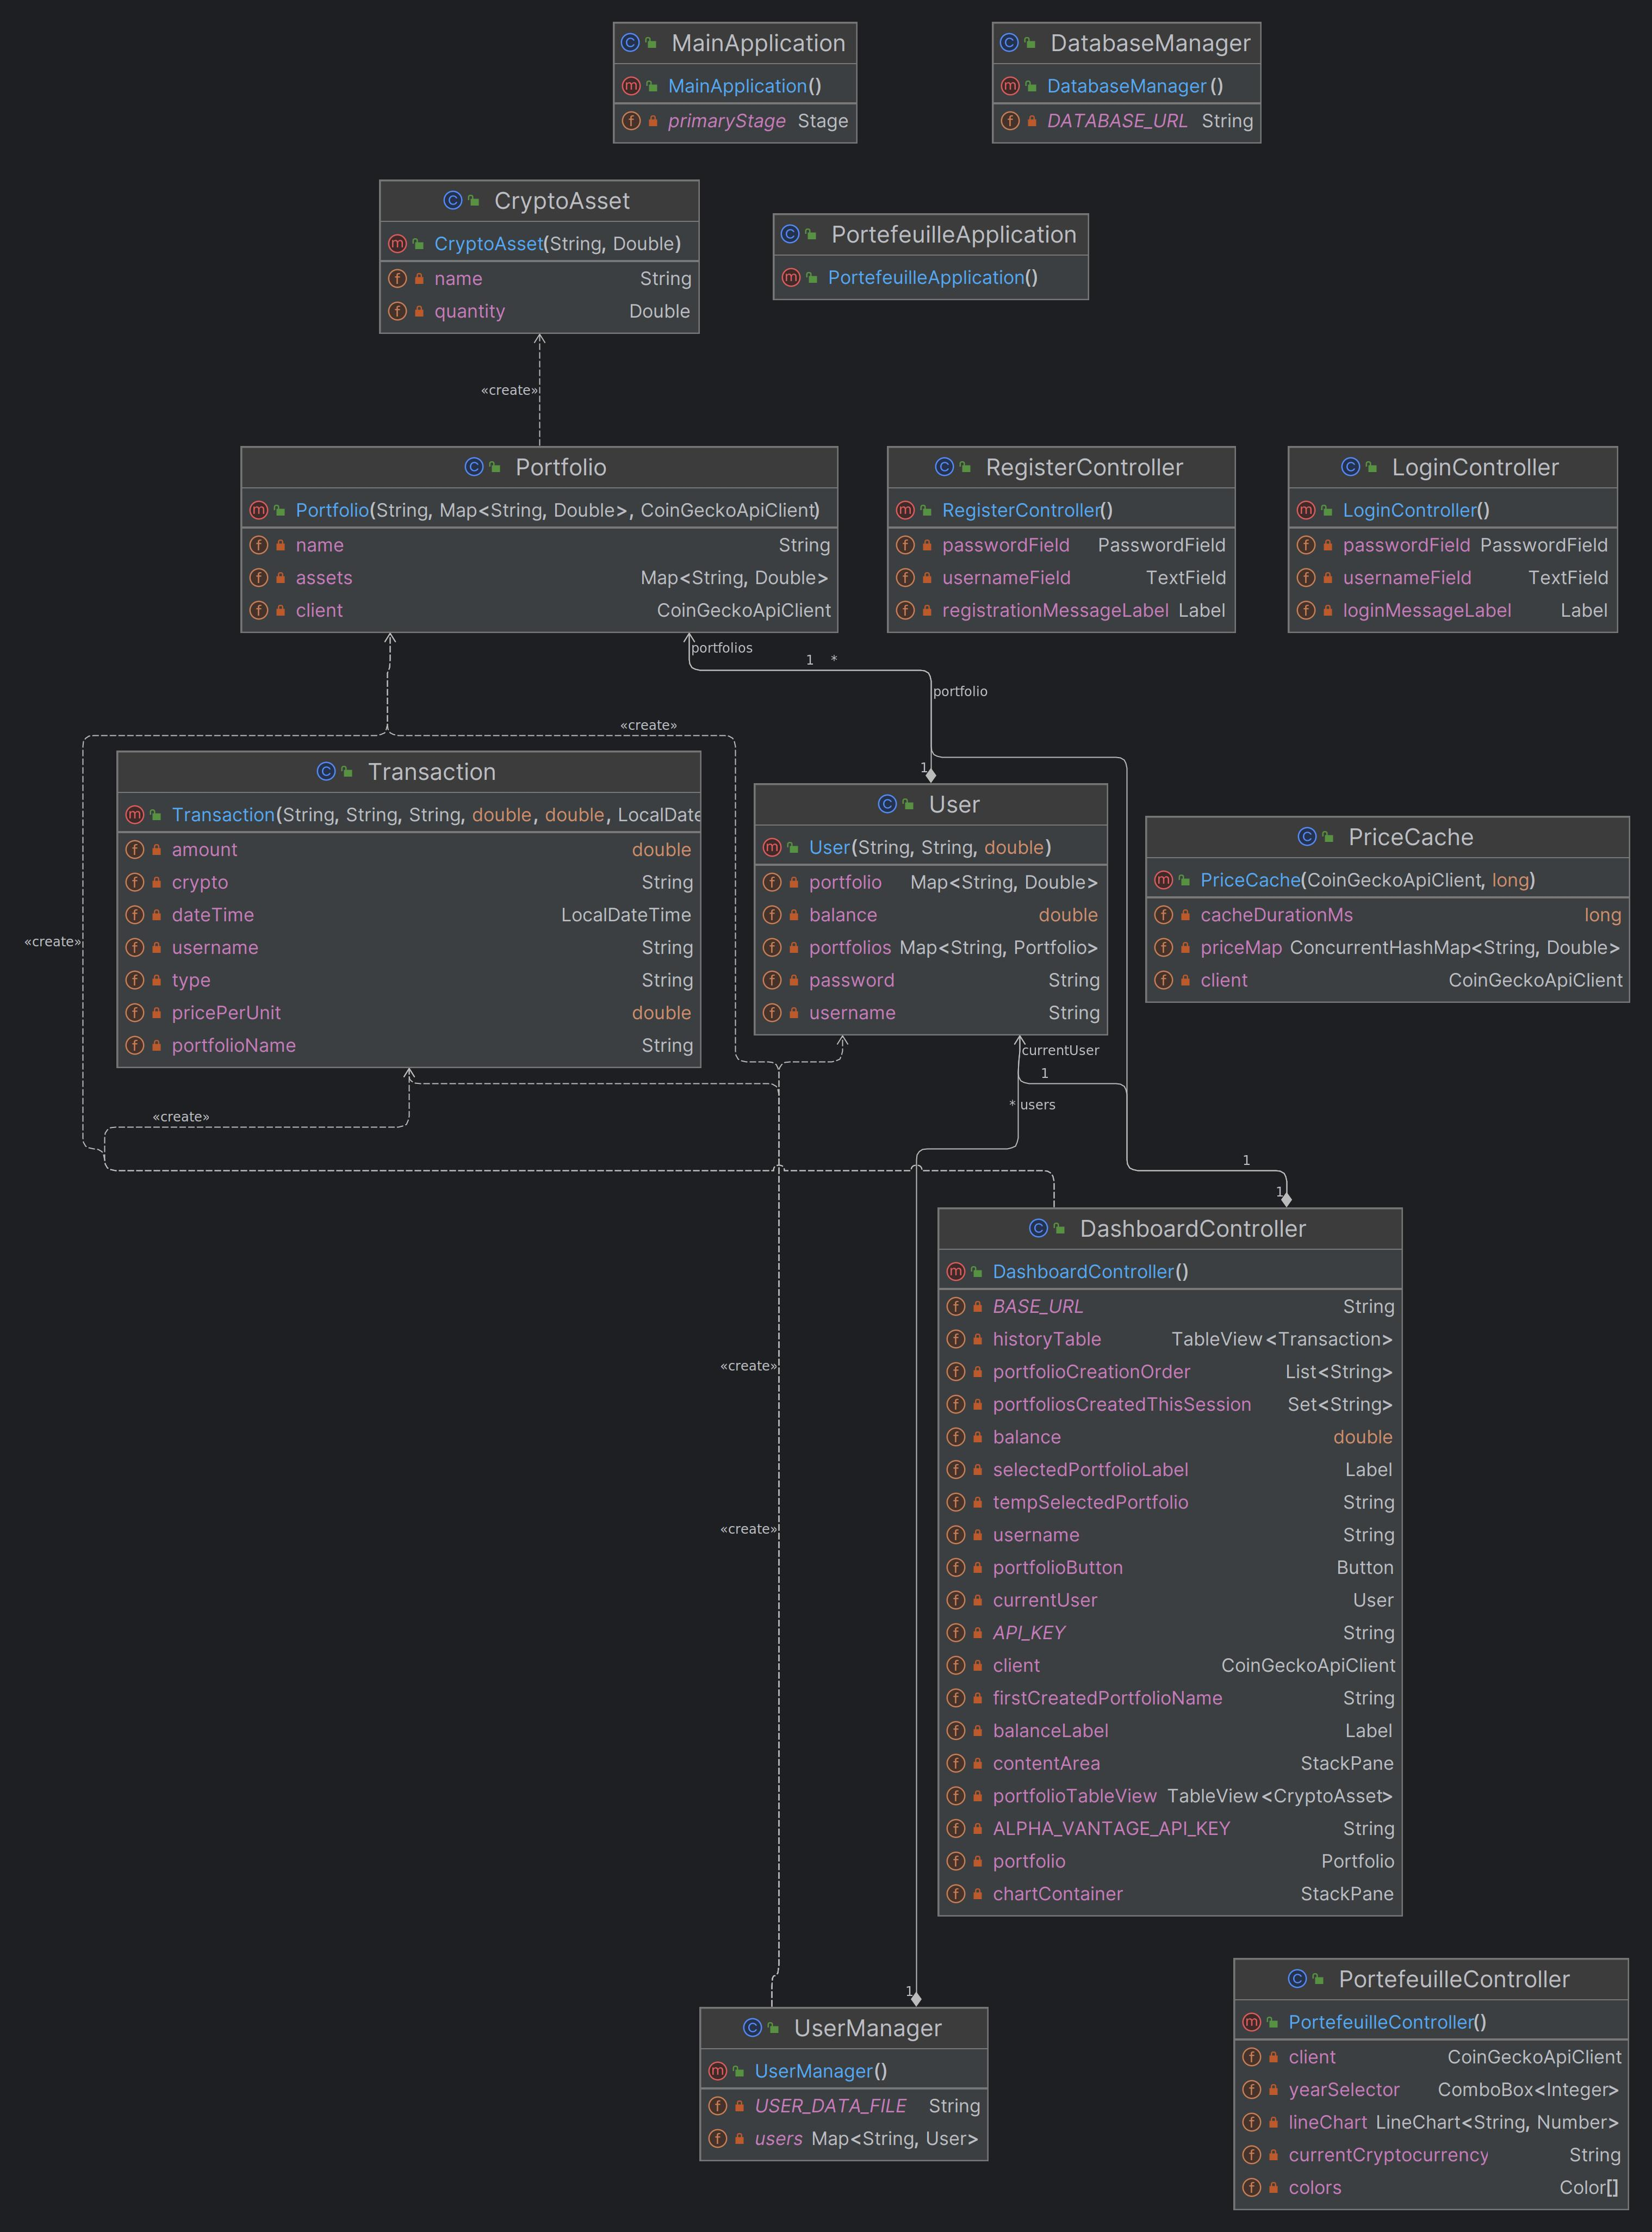
\includegraphics[width=0.7\linewidth]{UML1.jpg}
    \caption{Diagramme UML contenant les constructeurs et les variables.}
    \label{fig:enter-label}
\end{figure}
\newpage
\section{Description de la structure du projet}
\subsection{Structure interne}
Durant la phase de planification, la structure du projet fut l'une de nos priorités. Pour ce faire, nous avons choisi d'adopter une structure avec un tableau de bord centralisant les diverses fonctionnalités de notre projet. De plus, nous avons essayé de suivre le pattern M.V.C. (Model View Controller) pour certaines fonctionnalités, cela nous a permis de pouvoir tester les fonctionnalités sans avoir à se connecter à chaque fois. Chaque fichier de type Controller a un fichier FXML qui lui est associé. De plus, nous avons utilisé un fichier XML afin de pouvoir gérer les dépendances sous Maven. Notre projet est structuré de manière à faciliter l'accès et l'organisation des composants. Du point de vue de la structure des fichiers, les codes sont organisés au sein d'un dossier (package) \textbf{src} qui se divisent en deux sections principales. \begin{enumerate}
    \item  La première avec les ressources c'est-à-dire les fichiers FXML et les images.
    \item La seconde contient les codes des classes Java. Cette dernière section est elle même séparée en deux sections différentes : La première consacrée à l'API Coingecko. La seconde contenant le code des classes Java propre à notre projet.
    \end{enumerate}

\begin{figure}[H]
    \centering
    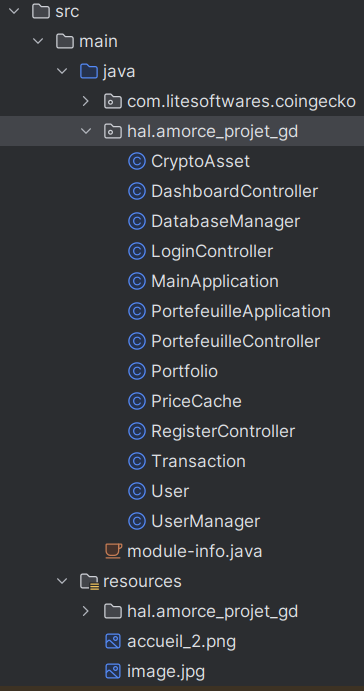
\includegraphics[width=0.25\linewidth]{Ajout.png}
    \caption{Structure interne du projet.}
    \label{fig:enter-label}
\end{figure}

\newpage
\subsection{Structure de l'interface}
Concernant la structure de l'interface de notre projet, nous avons décider de mettre toutes nos fonctionnalités sur une barre verticale (VBox) à gauche de notre tableau de bord. Grâce à cette structure nous avons une bonne visualisation générale de l'intégralité des fonctionnalités que nous avons réalisées. Ensuite, l'écran à droite de cette barre verticale sert d'affichage. Nous avons trouvé que de cette manière, il était plus simple et clair pour l'utilisateur de n'avoir qu'une seule et même interface.\\

Ensuite, pour les boutons, étant donné que nous avions beaucoup de fonctionnalités à implémenter, nous avons décidé d'en rassembler certains dans un menu déroulant. Par exemple, nous avons concentrer les boutons dupliquer, supprimer, ajouter et choix du portefeuille dans un même bouton appelé 'Options du portefeuille'. Nous avons aussi organisé l'UI sous forme de section (Portefeuille, Investir, Cryptos et Action) pour une meilleure lisibilité. Pour réalisé l'UI du programme nous avons utilisé un fichier styles.css qui régis les règles esthétiques des boutons, tableaux et menus déroulants. Cela nous a permis d'enrichir l'aspect visuel de l'application tout en réduisant la taille des fichiers fxml. Nous avons ainsi pu ajouter des fonctions de customisations précises comme des modifications esthétiques lorsque le curseur survol des boutons cliquables ou par exemple la couleur de la sélection des lignes des tableaux.


\begin{figure}[H]
    \centering
    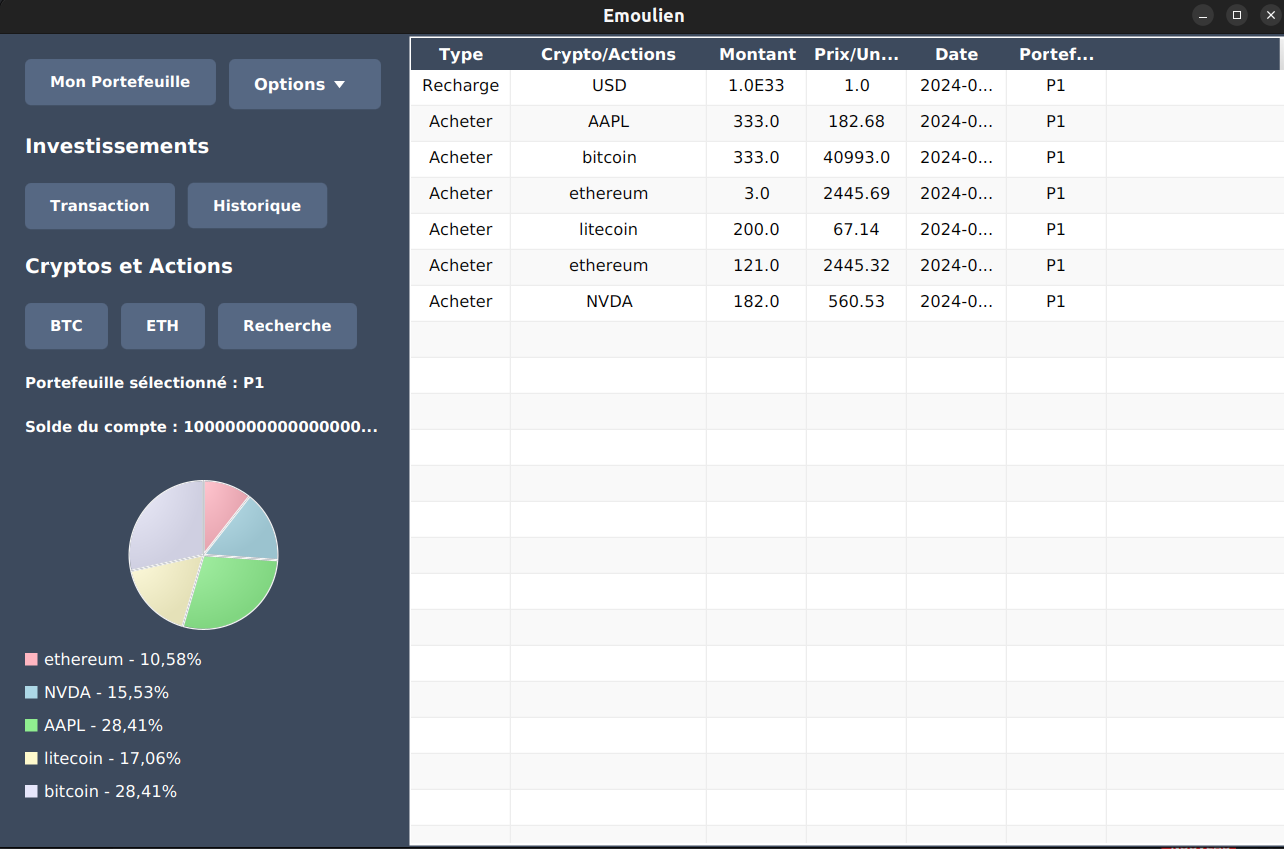
\includegraphics[width=0.75\linewidth]{dash1.png}
    \caption{Interface du dashboard et de l'historique}
    \label{fig:enter-label}
\end{figure}

\newpage
\section{Déroulement du projet}
Avant de commencer à coder, nous avons procéder en plusieurs étapes. Tout d'abord, nous avons regarder les différentes fonctionnalités du projet qui étaient à réaliser afin de comprendre au mieux ce qui était attendu. Ensuite, nous avons classé en terme de difficulté les différentes fonctionnalités du projet. Faire cette classification nous a permis non seulement de visualiser l'ensemble des attentes mais également de pouvoir commencer par des fonctionnalités qui étaient abordables afin de ne pas rester bloquer sur une fonctionnalité difficile et ne pas avancer. 
Dans cette partie, nous aborderons donc de la répartition des tâches que nous avons adopté durant ce projet, puis les difficultés rencontrées ainsi que les solutions à ces problèmes.

\
\subsection{Répartition des tâches}

Tout d'abord, concernant la répartition des tâches, nous avons procéder d'une manière bien précise. Comme énoncé précédemment, nous avons classifié par intensité de travail chaque aspect du projet. Une fois cette classification faite, nous avions pour méthode de commencer par la première fonctionnalité à implémenter. Nous essayons tous de travailler sur cette fonctionnalité. Lorsqu'une personne arrive à faire fonctionner son code, elle le met sur Github et le reste du groupe partait donc du code de la personne ayant réussi afin de pouvoir commencer la deuxième. Nous avons adopter ce processus du début à la fin du projet. Nous avons trouvé que cette méthode était la plus efficace afin d'avoir un maximum de productivité. En effet, lorsque chacun avance sur une partie du projet, il est possible que les deux codes ne soient pas compatibles ce qui provoquerait donc une énorme perte de temps afin de rendre les deux codes compatibles. \\

Enfin, en ce qui concerne la soutenance et le rapport, nous nous sommes répartis les parties du rapport et nous avons présenté chaque partie que nous avons rédiger afin d'être le plus efficace possible. 



\subsection{Difficultés et solutions}

Ensuite, au cours du développement de ce projet nous avons rencontré plusieurs difficultés. Cette partie abordera donc les différentes difficultés rencontrées et la solution que nous avons trouvé pour pallier ces problèmes. \\

Tout d'abord, trouver les classes qui allaient constituer notre projet était compliqué. En effet, ce projet était le premier durant lequel nous devions choisir nous même le nom des classes et l'utilité de chaque classe. La réalisation du diagramme nous a beaucoup aidé a visualiser les différentes classes qui allaient constituer notre projet. En outre, nous avons trouvé que interagir avec l'API (Coin gecko) était compliqué. Cependant, en faisant des recherches sur internet ainsi que grâce au cours du professeur nous expliquant brièvement comment interagir et importer coin gecko, nous avons finalement pu réussir. Nous avons été limité par l'API qui n'autorise que 5 requêtes toutes les 5 minutes donc certaines idées on dû être abandonnées. Enfin, une difficulté qui nous a posé problème au cours du projet était l'ajout de fonctionnalités. Au fur et à mesure de l'ajout de fonctionnalités, nous avons trouvé que parfois ajouter une fonctionnalité provoquait des bugs dans une autre fonctionnalité. Il était donc compliqué de rajouter des fonctionnalités au fur et à mesure de l'avancement du projet. La sauvegarde via une base de données SQL, fut également une tache difficile, nous avions d'abord essayé plusieurs autres méthodes de sauvegarde qui n'aboutissaient pas. Puis, après diverses recherches, nous en avons conclus que la base de données SQL était la meilleure option. Enfin, nous avons été confronté à une autre difficulté trouvée à la fin de notre projet. En effet, nous nous sommes rendus compte que l'API Coingecko pouvait nous fournir uniquement des valeurs de cryptomonnaies, toutes les valeurs liées à des actions d'entreprises étaient absurdes. Pour résoudre ce problème, nous avons du procéder à l'ajout d'une nouvelle API : Alpha Vantage qui nous permet d'obtenir les valeurs des actions d'entreprises. Cependant travailler avec cette API a été un nouveau problème supplémentaire puisque nous somme limités à 25 requêtes par jour. Nous avons donc organisé des sessions produit où l'un d'entre nous utilisait toutes ses requêtes pour tester les bugs de l'application et le reste de la journée on limitait au maximum les requêtes pour faire un test final en fin de journée. \\

Ainsi, ce projet nous a permis de nous confronter à des problèmes et donc de savoir comme réagir face à ces derniers lors de projets futurs. 



\section{Conclusion : expérience acquise}

Ainsi, ce projet nous a permis d'acquérir de nouvelles compétences ou d'en approfondir certaines. Premièrement, ce projet nous a permis d'améliorer notre niveau en Java. En effet, en proposant un projet d'une difficulté élevé, cela nous a permis de nous dépasser et d'apprendre d'une manière ludique à coder en Java. Deuxièmement, ce projet nous a permis de mieux savoir s'organiser en équipe que ce soit en terme de communication ou encore de collaboration, ce projet nous sera utile dans nos projets futurs. Par ailleurs, la résolution de problèmes a constitué une grosse partie de notre projet. En effet, le fait de réfléchir en équipe aux différents problèmes que nous avons rencontré a été enrichissant. Ce projet a donc été bénéfique sur le plan mental comme sur le plan social et nous a permis d'améliorer nos compétences. 


\end{document}